\section{Auswertung}

\subsection{Bestimmung der Zeitkonstante eines RC-Glieds}

Wir verwenden die in Aufgabenteil 1 gemessenen Halbwertszeiten, um die Zeitkonstante nach Gleichung \eqref{eq:zeitkonst} zu berechnen. Den theoretischen Wert der Zeitkonstante ermitteln wir anhand der Formel $\tau = RC$ mit dem Widerstand $R$ und der Kapazität $C$. Die resultate der Berechnungen für alle vier Konfigurationen der RC-Schaltung sind \tabref{tab:a1_zeitkonst} zu entnehmen.

\renewcommand{\arraystretch}{1.5}
\begin{table}[H]
  \centering
  \caption{Messwerte und berechnete Größen der Zeitkonstante $\tau$.}
  \vspace*{1em}
  \begin{tabular}{| c | c | c | c | c | c |}
      \hline
      $C\ [\si{\nano\farad}]$ & $R\ [\si{\kilo\ohm}]$ & $f\ [\si{\hertz}]$ & $\tau_{\text{theo}}\  [\si{\second}]$ & $\tau_{\text{exp}}\ [\si{\second}]$ & Abw. \\
      \hline
      $470 \pm 47$ & $1.00 \pm 0.05$ & $165 \pm 1$ & $(47 \pm 6) \times 10^{-5}$ & $(43 \pm 15) \times 10^{-5}$ & $0.25\sigma$ \\
      \hline
      $4.70 \pm 0.47$ & $10.00 \pm 0.50$ & $165 \pm 1$ & $(4.7 \pm 0.6) \times 10^{-5}$ & $(6.49 \pm 0.15) \times 10^{-5}$ & $3.29\sigma$ \\
      \hline
      $47.00 \pm 4.70$ & $1.00 \pm 0.05$ & $165 \pm 1$ & $(4.7 \pm 0.6) \times 10^{-5}$ & $(4.91 \pm 0.15) \times 10^{-5}$ & $0.38\sigma$ \\
      \hline
  \end{tabular}
  \label{tab:a1_zeitkonst}
\end{table}
\renewcommand{\arraystretch}{1}

\abbref{fig:aufgabe1_rc_signalverlauf} zeigt exemplarisch den Spannungsverlauf für die letzte angegebene Schaltungskonfiguration. 


\begin{figure}[H]
  \centering
  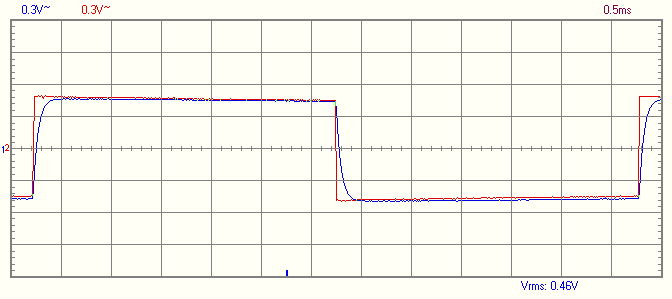
\includegraphics[width=.8\textwidth]{files/aufgabe1_rc_signalverlauf.png}
  \caption{Spannungsverlauf am Oszilloskop des RC-Glieds für $C = 47\si{\nano\farad}$, $R = 1 \si{\kilo\ohm}$. In Rot dargestellt die Eingangsspannung $U_E$, in Blau die Ausgangsspannung $U_C$, abgenommen über den Kondensator.}
  \label{fig:aufgabe1_rc_signalverlauf}
\end{figure}

\subsection{RC-Glied als Integrator und Differentiator}

Wie bereits dem Versuchsprotokoll zu entnehmen können wir beim Aufbau der RC-Schaltung als Integrator beobachten, dass sich das Ausgangssignal bei Erhöhung des Widerstandes immer stärker dem Integral des Eingangssignals annähert. So formt ein eingehendes Rechteckssignal eine Dreiecksfunktion als Ausgangssignal, aus einem eingehenden Dreieckssignal ergibt sich ein Sinussignal, wie in \abbref{fig:aufgabe2_integral_dreieck} zu sehen.

\begin{figure}[H]
  \centering
  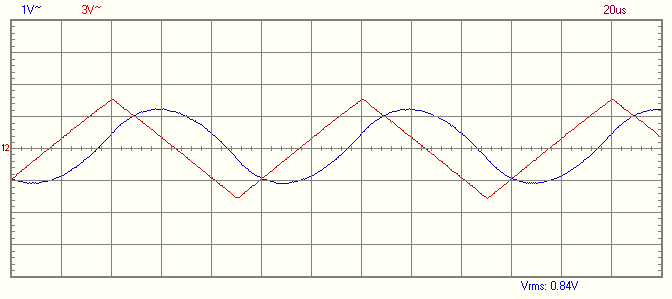
\includegraphics[width=.8\textwidth]{files/aufgabe2_integral_dreieck.png}
  \caption{Spannungsverlauf beim Betrieb der RC-Schaltung als Integrator. In Rot dargestellt die dreiecksförmige Eingangsspannung $U_E$, in Blau die Ausgangsspannung $U_C$, abgenommen über den Kondensator.}
  \label{fig:aufgabe2_integral_dreieck}
\end{figure}

Ähnliche Beobachtungen können wir beim Betrieb des RC-Glieds als Differentiator machen. Bei Justierung des Widerstandes ergibt sich hierbei beispielsweise aus einem eingehenden Dreieckssignal ein ausgehendes Rechteckssignal, siehe \abbref{fig:aufgabe2_differentiator_dreieck}. Geben wir durch den Funktiongenerator ein Signal in der Form einer Gauß'schen Normalverteilung ein, so ergibt sich auch hiervon die entsprechende Ableitung, zu sehen in \abbref{fig:aufgabe2_differentiator_gauss}.


\begin{figure}[H]
  \centering
  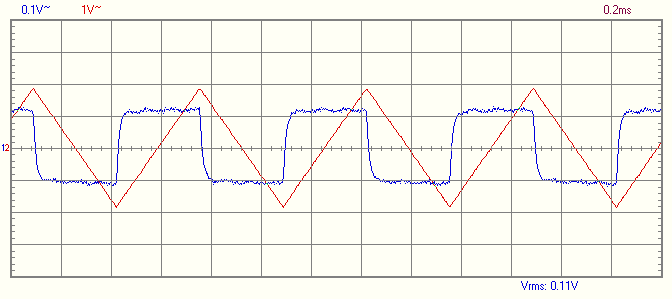
\includegraphics[width=.8\textwidth]{files/aufgabe2_differentiator_dreieck.png}
  \caption{Spannungsverlauf beim Betrieb der RC-Schaltung als Differentiator. In Rot dargestellt die dreiecksförmige Eingangsspannung $U_E$, in Blau die Ausgangsspannung $U_R$, abgenommen über den Widerstand.}
  \label{fig:aufgabe2_differentiator_dreieck}
\end{figure}

\begin{figure}[H]
  \centering
  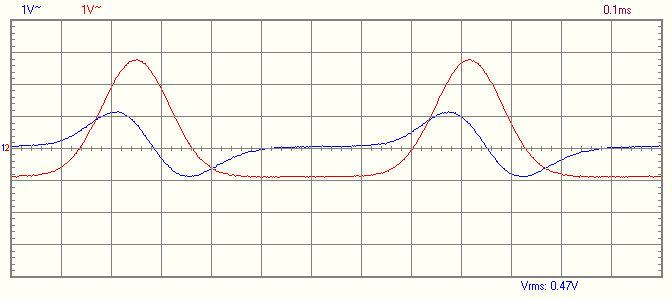
\includegraphics[width=.8\textwidth]{files/aufgabe2_differentiator_gauss.png}
  \caption{Spannungsverlauf beim Betrieb der RC-Schaltung als Differentiator. In Rot dargestellt die Eingangsspannung $U_E$, in Blau die Ausgangsspannung $U_R$, abgenommen über den Widerstand.}
  \label{fig:aufgabe2_differentiator_gauss}
\end{figure}


\subsection{Frequenz- und Phasengang eines RC-Glied}

\small \textit{Für diesen Aufgabenteil ist anzumerken, dass wir bei der Durchführung leider den Frequenzgang nicht ab $100\si{\hertz}$ wie vorgegeben, sondern erst ab $1\si{\kilo\hertz}$ aufgezeichnet haben. Damit ist die lineare Interpolation, welche in der Auswertung gefordert wird, nicht zielführend und wird im folgenden deshalb ausgelassen. Außerdem ist unsere abgelesene Grenzfrequenz des Tiefpassfilters jenseits von Gut und Böse.}
\normalsize

In diesem Teil der Auswertung bestimmen wir aus dem aufgezeichneten Frequenzgängen eines Tief- und Hochpassfilters die Grenzfrequenz bestimmen. Wie in den theoretischen Grundlagen erklärt, ist die Grenzfrequenz der Filterschaltung dadurch zu erkennen, dass bei ihr die Amplitude um den Faktor $\flatfrac{1}{\sqrt{2}}$ abgefallen ist. Mit der \textit{Curser}-Funktion des Oszilloskops können wir damit eine Grenzfrequenz von $(9.46 \pm 0.02)\si{\kilo\hertz}$ für den Tiefpassfilter und eine Grenzfrequenz von $(3.31 \pm 0.02) \si{\kilo\hertz}$ für den Hochpassfilter ablesen. Die untenstehenden Abbildungen zeigen noch einmal die Frequenzgänge des Tiefpassfilters (\ref{fig:aufgabe3_tiefpass}) und Hochpassfilters (\ref{fig:aufgabe3_hochpass}), jeweils mit dem Cursor an der Grenzfrequenz.


\begin{figure}[H]
  \centering
  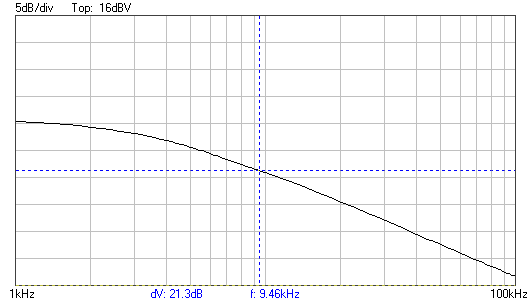
\includegraphics[width=.8\textwidth]{files/aufgabe3_tiefpass.png}
  \caption{Frequenzgang des Tiefpassfilters mit Cursor bei Grenzfrequenz}
  \label{fig:aufgabe3_tiefpass}
\end{figure}

\begin{figure}[H]
  \centering
  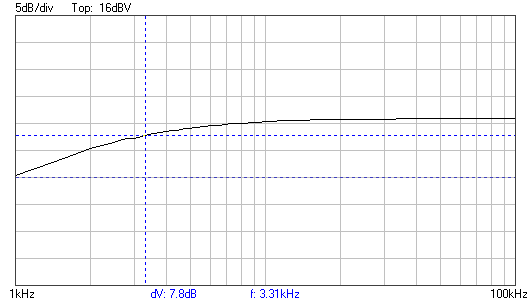
\includegraphics[width=.8\textwidth]{files/aufgabe3_hochpass.png}
  \caption{Frequenzgang des Hochpassfilters mit Cursor bei Grenzfrequenz}
  \label{fig:aufgabe3_hochpass}
\end{figure}

Neben der Aufzeichnung des Frequenzgangs haben wir für den Hochpassfilter zusätzlich den Phasengang manuell vermessen. Die Phase $\varphi$ ist in \abbref{fig:phaseshift_hp_fit} über der Frequenz aufgetragen. Die Grenzfrequenz bestimmen wir nun durch Ablesen Frequenz bei einer Phase von $45\si{\degree}$. Die Phase zeigt, abhängig von der Frequenz, einen logarithmisch abfallenden Verlauf auf. Um den Wert bei $45\si{\degree}$ interpolieren zu können fitten wir eine abfallende Exponentialfunktion der Form
\begin{align}
  f(x; A,\lambda,c) = A \cdot \e{- \lambda x} + c
\end{align}
an die Datenpunkte an. Die optimierten Werte der Parameter sind ebenfalls der \abbref{fig:phaseshift_hp_fit} zu entnehmen.


\begin{figure}[H]
  \centering
  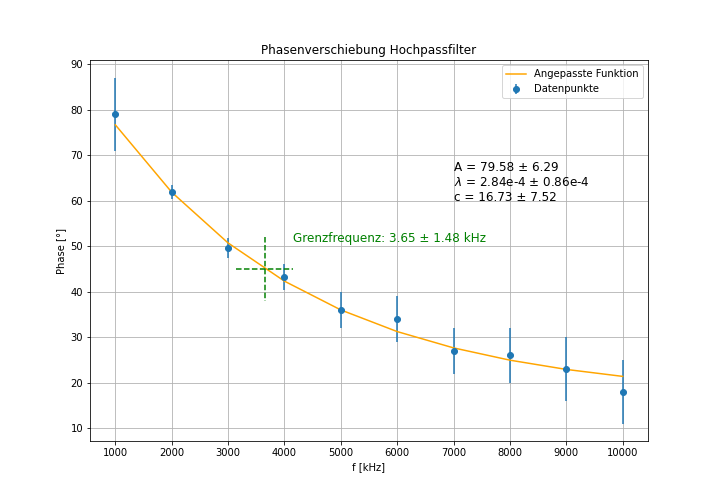
\includegraphics[width=.8\textwidth]{files/phaseshift_hp_fit.png}
  \caption{Phasengang des Hochpassfilters mit exponentiellem Fit und Grenzfrequenz bei $45\si{\degree}$.}
  \label{fig:phaseshift_hp_fit}
\end{figure}


Durch elementares Umformen bestimmen wir die Umkehrfunktion von $f$, um damit die Grenzfrequenz berechnen zu können. Für diese gilt
\begin{align}
  f^{-1}(\varphi; A, \lambda, c) = - \frac{1}{\lambda} \ln(\frac{\varphi - c}{A}) = f_{\mathrm{Grenz}}.
\end{align}
Nach der gauß'schen Fehlerfortpflanzung gilt für der Fehler des damit berechneten Wertes
\begin{align}
  \Delta f_{\mathrm{Grenz}} = \sqrt{\qty(\frac{1}{\lambda A} \ln(\frac{\varphi - c}{A}) \cdot \Delta A)^{2} + \qty(\frac{1}{\lambda^2} \ln(\frac{\varphi - c}{A}) \cdot \Delta \lambda)^{2} + \qty(\frac{1}{\lambda(\varphi - c)} \cdot \Delta c)^{2}}.
\end{align}

Damit können wir aus der Funktion eine Grenzfrequenz von
\begin{align}
  f_{\mathrm{Grenz}} = (3.65 \pm 1.48) \si{\kilo\hertz}
\end{align}
interpolieren. Diese ist ebenfalls in Grün in \abbref{fig:phaseshift_hp_fit} markiert. Von der zuvor vermessenen Grenzfrequenz weicht diese um etwa $2.47\sigma$ ab, was innerhalb des $3\sigma$-Bereichs noch als eine nicht signifikante Abweichung angesehen werden kann.

Nach der Theorie gilt für die Grenzfrequenz des Hoch- bzw. Tiefpassfilter die Gleichung
\begin{align}
  f_G &= \frac{1}{CR} \qty[\times \frac{1}{2 \pi}].
\end{align}
Setzen wir für die entsprechenden Werte der Kapazität $C = 47\si{\nano\farad}$ und des Widerstands $R = 1\si{\kilo\ohm}$ ein, so erhalten wir dazu einen Wert von
\begin{align}
  f_{Grenz} = (3.4 \pm 0.4)\si{\kilo\hertz}.
\end{align}

Dieser weicht um $0.21\sigma$ vom ausgemessenen Wert aus dem ersten Teil und um $2.47\sigma$ vom interpolierten Wert ab.

\subsection{Frequenzgang eines Serienschwingkreises}

Für diesen Aufgabenteil betrachten wir erstmals einen Serienschwingkreis, also eine Schaltung bestehend aus Kondensator, Widerstand und Spule. Im ersten Schritt möchten wir die Induktivität der verbauten Spule berechnen, dazu ziehen wir \eqref{eq:rlc_omega_r} hinzu und stellen diese um nach
\begin{align}
  L &= \frac{1}{\omega_R^2 C}
\end{align}
mit der Kapazität $C$, sowie gemessenen Resonanzfrequenz $\omega_R$, welche wir zuvor durch den Faktor $2\pi$ noch in eine Kreisfrequenz umrechnen. In der Durchführung haben wir die Messungen für drei unterschiedliche Widerstände durchgeführt und dafür die Frequenzgänge, zu sehen in \abbref{fig:aufgabe4_frequenzgang_schwingkreis} aufgezeichnet. Aus den Maxima der Frequenzgänge haben wir dann die Resonanzfrequenz abgelesen.

\begin{figure}[H]
  \centering
  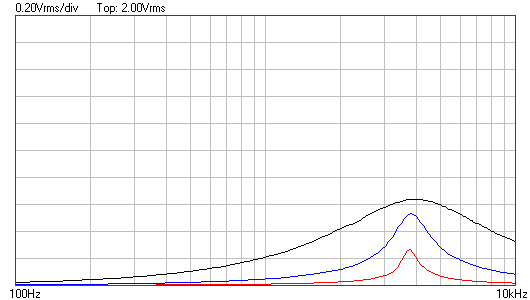
\includegraphics[width=.8\textwidth]{files/aufgabe4_frequenzgang_schwingkreis.png}
  \caption{Frequenzgang des RLC-Schwingkreises für drei verschiedene Widerstände.}
  \label{fig:aufgabe4_frequenzgang_schwingkreis}
\end{figure}

Für die drei Frequenzen berechnen wir jeweils eine Induktivität und nehmen davon den Mittelwert von
\begin{align}
  L = (3.63 \pm 0.22) \cdot 10^{-2} \si{\henry}
\end{align}
als Wert für die Induktivität der Spule.

Als Nächstes betrachten wir die Verluste, welche in der Spule durch ihren eigenen ohmschen Widerstand, magnetische Verluste des Spulenkerns, sowie den Skineffekt entstehen. Um diese Verluste zu quantifizieren, nehmen wir die Existenz eines weiteren Verlustwiderstandes $R_V$ in der Schaltung an. \eqref{eq:rlc_bandbreite} stellt einen Zusammenhang zwischen dem Gesamtwiderstand und der Bandbreite der RLC-Schaltung her, welchen wir entsprechend umstellen zu
\begin{align}
  R + R_V = \Delta \omega \cdot L.
\end{align}

Wie im Theorieteil beschrieben stellt das RLC-Glied im Resonanzfall bei $\omega_R$ einen Kurzschluss dar, da die Impedanz des LC-Gliedes verschwindet. Für das Verhältnis von Ein- und Ausgangsspannung, letztere abgenommen am Widerstand $R$, ergibt sich somit der einfache Zusammenhang
\begin{align}
  U_A = \frac{R}{R + R_V} U_E
\end{align}
und somit durch
\begin{align}
  R + R_V &= R \frac{U_E}{U_A}
\end{align}
eine weitere Formel, um den Gesamtwiderstand zu berechnen. Die folgende \tabref{tab:verlustwiderstand} zeigt nun die in den drei Messgängen aufgezeichneten Werte der Ein- und Ausgangsspannung $U_E$ und $U_A$, der Resonanzfrequenz $\omega_R$, sowie der Bandbreite $\Delta \omega$. Als Induktivität verwenden wir den zuvor berechneten Mittelwert. Weiter enthält die Tabelle die berechneten Werte für $R + R_V$, den verwendeten Widerstand, sowie deren Differenz, also die Verlustleistung $R_V$.

\renewcommand{\arraystretch}{1.5}
\begin{table}[H]
  \centering
  \caption{Messwerte und Resultate für die Berechnung des Verlustwiderstandes.}
  \vspace*{1em}
  \begin{tabular}{|c|c|c|c|c|}
    \hline
    \multicolumn{2}{|c|}{$R\,[\si{\ohm}]$} & $1000 \pm 50$ & $220 \pm 11$ & $47.0 \pm 2.4$ \\
    \hline
    \multicolumn{2}{|c|}{$U_E\,[\si{\volt}]$} & $0.661 \pm 0.001$ & $0.650 \pm 0.001$ & $0.627 \pm 0.001$ \\
    \hline
    \multicolumn{2}{|c|}{$U_A\,[\si{\volt}]$} & $0.640 \pm 0.020$ & $0.530 \pm 0.020$ & $0.270 \pm 0.020$ \\
    \hline
    \multicolumn{2}{|c|}{$\Delta \omega\,[\si{\per\second} \cdot 10^3]$} & $30.91 \pm 0.19$ & $8.11 \pm 0.19$ & $3.52 \pm 0.19$ \\
    \hline
    \hline
    \multirow{2}{*}{Aus Bandbreite} & $R + R_V\,[\si{\ohm}]$ & $1123 \pm 650$ & $294 \pm 171$ & $128 \pm 75$ \\
    \cline{2-5}
    & $R_V\,[\si{\ohm}]$ & $123 \pm 652$ & $74 \pm 171$ & $80 \pm 75$ \\
    \hline
    \hline
    \multirow{2}{*}{Aus Amplituden} & $R + R_V\,[\si{\ohm}]$  & $1033 \pm 61$ & $270 \pm 17$ & $109 \pm 10$ \\
    \cline{2-5}
    & $R_V\,[\si{\ohm}]$ & $33 \pm 79$ & $49.811 \pm 21$ & $62.144 \pm 11$ \\
    \hline
  \end{tabular}
  \label{tab:verlustwiderstand}
\end{table}
\renewcommand{\arraystretch}{1}

\textit{Ich habe mir herausgenommen, die Aufgaben etwas umzusortieren.}

\subsection{Bestimmung der Dämpfungskonstanten eines freien, gedämpften Schwingkreises}

Anstatt eines kontinuierlichen Signals geben wir nun mit dem Funktionsgenerator ein Rechteckssignal in den Serienschwingkreis ein, um wiederholt einen auslaufenden Schwingungprozess anzustoßen (vgl. \abbref{fig:aufgabe6_schwingung_gedaempft}).

\begin{figure}[H]
  \centering
  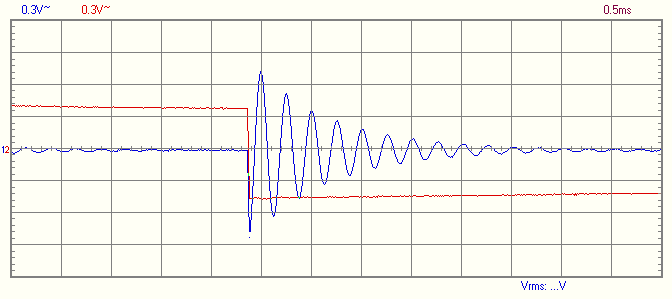
\includegraphics[width=.8\textwidth]{files/aufgabe6_schwingung_gedaempft.png}
  \caption{Gedämpfte Schwingung}
  \label{fig:aufgabe6_schwingung_gedaempft}
\end{figure}

Für je zwei benachbarte Amplituden der Schwingung berechnen wir nun das logarithmische Dekrement nach Formel \eqref{eq:log_dekr}.

\renewcommand{\arraystretch}{1.5}
\begin{table}
  \centering
  \caption{Logarithmisches Dekrement für je zwei benachbarten Amplituden der gedämpften Schwingung.}
  \begin{tabular}{c|c|c}
    $A_n\,[\si{\volt}]$ & $A_{n+1}\,[\si{\volt}]$ & $\Lambda$\\\hline
    $0.74 \pm 0.02$ & $0.50 \pm 0.02$ &	$0.39 \pm 0.05 $\\
    $0.50 \pm 0.02$ & $0.36 \pm 0.02$ &	$0.33 \pm 0.07 $\\
    $0.36 \pm 0.02$ & $0.26 \pm 0.02$ &	$0.33 \pm 0.10 $\\
    $0.26 \pm 0.02$ & $0.18 \pm 0.02$ &	$0.37 \pm 0.14 $\\
    \hline\hline
    \multicolumn{2}{c}{Mittelwert} & $0.35 \pm 0.05$\\\hline
  \end{tabular}
\end{table}
\renewcommand{\arraystretch}{1}

Für Periodendauer einer Schwingung haben wir einen Wert von $T = 0.26 \pm 0.02\si{\milli\second}$ gemessen. Diesen verwenden wir nun, um über den zweiten Teil der \eqref{eq:log_dekr} die Dämpfungskonstante $\delta$ beziehungsweise den Gesamtwiderstand nach
\begin{gather}
  \Lambda = \delta T = \frac{R}{2L} T \iff R = \frac{2 \Lambda L}{T}
  \intertext{mit Fehler}
  \Delta R = R \cdot \sqrt{\relerrsq{\Lambda} + \relerrsq{L} + \relerrsq{T}}
\end{gather}
zu berechnen. Unter anderem ziehen wir die berechnete Induktivität $L$ aus dem vorherigen Abschnitt hinzu. Damit erhalten wir einen Wert von
\begin{align}
  R = (99 \pm 60)\,\si{\ohm}.
\end{align}
Bei diesem handelt es sich wieder um den Gesamtwiderstand der RLC-Schaltung, also mit dem einberechneten Verlusten $R_V$ durch die Spule. Vergleichen wir den hier berechneten Wert mit dem Wert des vorherigen Abschnitts ($(128 \pm 75) \,\si{\ohm}$), verzeichnen wir eine Abweichung von etwa $0.31\sigma$.

\subsection{Resonanzüberhöhung}
Wir betrachten nun die Frequenzgänge der einzelnen Bauteile im RLC-Serienschwingkreis genauer. Diese sind gemeinsam in \abbref{fig:aufgabe5_resonanzueberhoehung} geplottet: In Rot der Frequenzgang des Kondensators, in Blau der Frequenzgang der Spule und in Schwarz der Frequenzgang des Widerstandes. Deutlich zu erkennen ist im Plot die Resonanzüberhöhung in den Frequenzgängen des Kondensators und der Spule.


\begin{figure}[H]
  \centering
  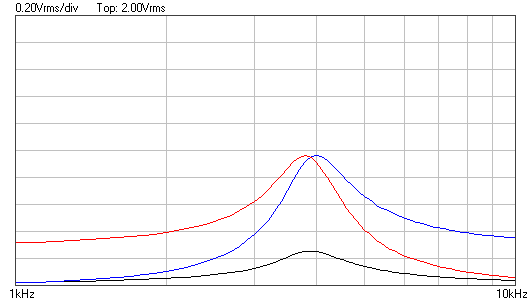
\includegraphics[width=.8\textwidth]{files/aufgabe5_resonanzueberhoehung.png}
  \caption{Frequenzgänge der einzelnen Bauteile Kondensator (rot), Spule (blau) und Widerstand (schwarz) im RLC-Serienschwingkreis.}
  \label{fig:aufgabe5_resonanzueberhoehung}
\end{figure}

Wir möchten nun unsere vermessenen Resonanzfrequenzen mit den entsprechenden theoretischen Werten vergleichen. Dazu berechnen wir zunächst die Dämpfungskonstante nach der Formel aus dem vorherigen Abschnitt zu
\begin{align}
  \delta = (3028 \pm 1758)\si{\per\second}.
\end{align}

Weiter berechnen wir die Resonanzfrequenz des Widerstandes nach \eqref{eq:rlc_omega_r} zu
\begin{align}
  \omega_R = (3910 \pm 20)\si{\per\second}.
\end{align}

Die Resonanzfrequenz des Kondensators berechnen wir mit der Formel \eqref{eq:rlc_omega_c}. Für den Fehler des Ergebnisses gilt hierbei
\begin{align}
  \Delta \omega_C = \sqrt{\qty(\frac{\omega_R \Delta \omega_R}{\omega_C})^2 + \qty(\frac{\delta \Delta \delta}{\omega_C})^2}.
\end{align}
Die Formel für die Resonanzfrequenz der Spule \eqref{eq:rlc_omega_l} ist dazu sehr ähnlich. Ihr Fehler berechnet sich nach der gleichen Formel wie beim Kondensator, wir ersetzen lediglich $\omega_C$ durch $\omega_L$. \tabref{tab:omega_vergleich} enthält nun die berechneten Werte, die gemessenen Werte, sowie die berechnete Abweichung.

\renewcommand{\arraystretch}{1.5}
\begin{table}[H]
  \centering
  \caption{Vergleich der gemessenen und theoretisch vorhergesagten Werte der Resonanzfrequenzen der Bauteile im RLC-Serienschwingkreis.}\vspace*{0.5em}
  \label{tab:omega_vergleich}
  \begin{tabular}{|l|c|c|c|}
    \hline
    & $\omega_R\,[\si{\per\second}]$ & $\omega_C\,[\si{\per\second}]$ & $\omega_L\,[\si{\per\second}]$\\\hline
    Gemessener Wert & $3910 \pm 20$ & $3800 \pm 20$ & $4040 \pm 20$ \\\hline
    Theoretischer Wert & $3851 \pm 1131$ & $3791 \pm 1149$ & $3911 \pm 1114$\\\hline\hline
    Abweichung & $0.06\sigma$ & $0.009\sigma$ & $0.12\sigma$\\
    \hline
  \end{tabular}
\end{table}
\renewcommand{\arraystretch}{1}
\newpage
\subsection{Parallelschwingkreis-Bandsperre}

Bevor wir zum anwendungsbezogenen Teil des Versuchs fortfahren, betrachten wir abschließend einen Parallelschwingkreis. Wir haben die Ausgangsspannung über den Widerstand abgegriffen erneut den Frequenzgang, zu sehen in \abbref{fig:aufgabe7_parallel_bandsperre}, aufgezeichnet.


\begin{figure}[H]
  \centering
  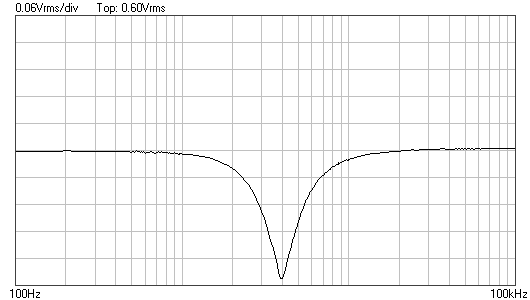
\includegraphics[width=.8\textwidth]{files/aufgabe7_parallel_bandsperre.png}
  \caption{Frequenzgang des RLC-Parallelschwingkreis.}
  \label{fig:aufgabe7_parallel_bandsperre}
\end{figure}

Aus dem Grafen können wir ablesen, dass die Bandsperre bei einer Resonanzfrequenz von $(3.94 \pm 0.02)\si{\kilo\hertz}$ greift. Die Ausgangsamplitude sinkt an dieser Stelle also auf $0\si{\volt}$ ab. Die Theorie sagt voraus, dass für die Resonanzfrequenz gilt $\omega_0 = \flatfrac{1}{\sqrt{LC}}$. Wir setzen die Werte für Kapazität und Induktivität ein und erhalten damit einen Wert von
\begin{align}
  f_0 &= (3851 \pm 1131) \si{\hertz}.
\end{align}
Dieser weicht um $0.078\sigma$ von dem von uns gemessenen Wert ab.
\newpage
\subsection{Signalformung}

In diesem Aufgabenteil betrachten wir nun die zuvor ausgiebig untersuchten Schaltungen im realitätsnahen Einsatz als Filter. Dafür generieren wir mit dem Frequenzgenerator ein Signal, welches sich aus drei überlagerten Sinussignale der Frequenzen $100\si{\hertz}$, $4\si{\kilo\hertz}$ und $8\si{\kilo\hertz}$, sowie weiteren weniger starken Störsignalen zusammensetzt. 

\subsubsection*{Ohne Filter}

Das zunächst ungefilterte Signal, sowie dessen Spektrum sind in \abbref{fig:aufgabe8_teil1_osz} zu sehen. Im Spektrum sind bereits jetzt ziemlich eindeutig die drei starken überlagerten Signalanteil bei den oben genannten Frequenzen zu erkennen. Im Oszilloskopbild liegen Aus- und Eingangsspannung ohne Filter genau übereinander, deshalb ist die Ausgabe in Grün dargestellt und es sind keine zwei Signale zu sehen.

\begin{figure}[H]
  \centering
  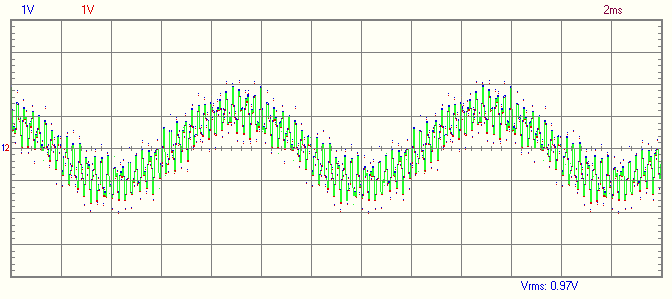
\includegraphics[width=.8\textwidth]{files/aufgabe8_teil1_osz.png}
  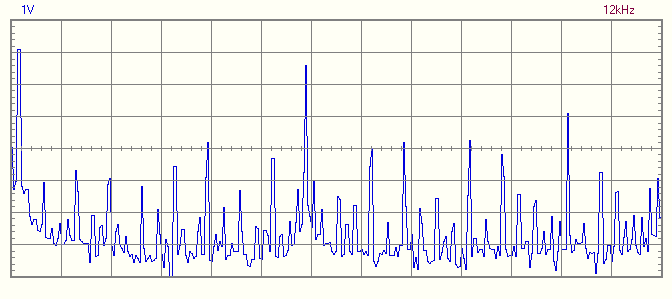
\includegraphics[width=.8\textwidth]{files/aufgabe8_teil1_spectrum.png}
  \caption{Ausgangsspannung und Frequenzspektrum des überlagerten Signals ohne Filter.}
  \label{fig:aufgabe8_teil1_osz}
\end{figure}

Ohne Filterung liegen die Amplituden der Signalanteile bei etwa

\renewcommand{\arraystretch}{1.5}
\begin{table}[H]
  \centering
  \begin{tabular}{c c}
    $100\si{\hertz}$: & $-3.06 \pm 0.02\,\mathrm{dBV}$,\\
    $4\si{\kilo\hertz}$: & $-8.06 \pm 0.02\,\mathrm{dBV}$,\\
    $8\si{\kilo\hertz}$: & $-22.13 \pm 0.02\,\mathrm{dBV}$.\\
  \end{tabular}
\end{table}
\renewcommand{\arraystretch}{1}

Wobei die Einheit dBV die gemessene Spannung in Bezug auf den Referenzwert von $1\si{\volt}$ angibt.

\newpage
\subsubsection*{Hochpassfilter}
Als Erstes betrachten wir das Signal gefiltert durch einen Hochpassfilter mit einem $220\si{\ohm}$ Widerstand und einem $470\si{\nano\farad}$ Kondensator. Im Frequenzspektrum in \abbref{fig:aufgabe8_teil2_hochpass} ist zu erkennen, dass der $100\si{\hertz}$-Signalanteil stark gedämpft wurde, während die anderen beiden, höherfrequente Signalanteile weitestgehend unverändert bleiben. Auch in der Signalformung des Ausgangssignals (blau) ist zu erkennen, dass die überliegende niedrigfrequente Sinusform stark abgeschwächt ist.


\begin{figure}[H]
  \centering
  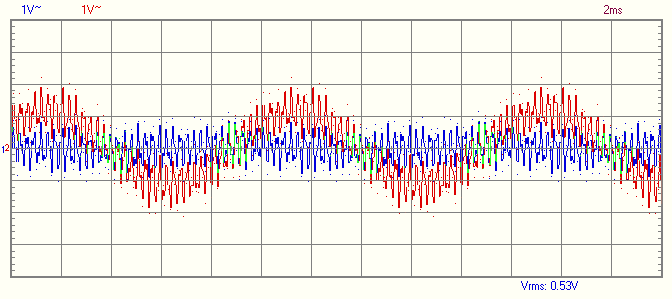
\includegraphics[width=.8\textwidth]{files/aufgabe8_teil2_hochpass_oszi.png}
  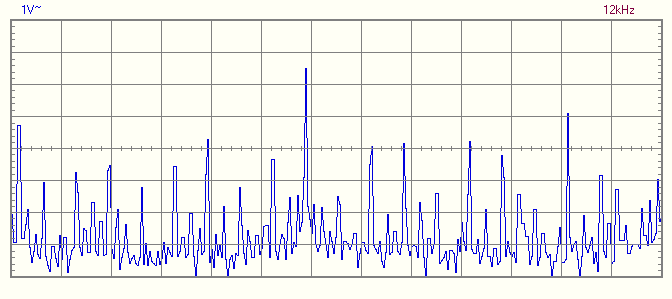
\includegraphics[width=.8\textwidth]{files/aufgabe8_teil2_hochpass_spectrum.png}
  \caption{Ein- (rot) und Ausgangsspannung (blau) und Frequenzspektrum des überlagerten Signals mit Hochpassfilter.}
  \label{fig:aufgabe8_teil2_hochpass}
\end{figure}

Um bei den verschiedenen Filterschaltungen die Dämpfungen berechnen und vergleichen zu können betrachten wir das Verhältnis zwischen der ungefilterten und der gefilterten Amplitude. \tabref{tab:dmpf_hochpass} fasst die Werte für den  Hochpassfilter zusammen.

\begin{table}[H]
  \centering
  \caption{Dämpfung der einzelnen Signalanteile beim $RC$-Hochpassfilter.}
  \vspace*{1em}
  \label{tab:dmpf_hochpass}
  \begin{tabular}{c|c|c|c}
    Signalanteil & Ungefilterte Amp. [dBV] & Gefilterte Amp. [dBV] & Dämpfung\\\hline
    100 Hz & $-3.06 \pm 0.02$ & $-26.81 \pm 0.02$ & $0.1141 \pm 0.0008$\\
    4 kHz & $-8.06 \pm 0.02$ & $-8.69 \pm 0.02$ & $0.928 \pm 0.004$\\
    8 kHz & $-22.13 \pm 0.02$ & $-22.44 \pm 0.02$ & $0.9862 \pm 0.0013$
  \end{tabular}
\end{table}


%4kHz ValErr(-8.06, 0.02) ValErr(-8.69, 0.02) ValErr(0.9275028768699656, 0.0031390427356231265)
%8kHz ValErr(-22.13, 0.02) ValErr(-22.44, 0.02) ValErr(0.9861853832442067, 0.0012517639252519503)
%100Hz ValErr(-3.06, 0.02) ValErr(-26.81, 0.02) ValErr(0.11413651622528907, 0.0007508336411163078)

\newpage
\subsubsection*{Tiefpassfilter}

Vertauschen wir Widerstand und Kondensator an der vorherigen Schaltung, so erhalten wir einen Tiefpassfilter. Wie zu erwarten, können wir im Spektrum (vgl. \abbref{fig:aufgabe8_teil2_tiefpass}) beobachten, dass nun der Signalanteil der niedrigen $100\si{\hertz}$-Frequenz den Filter unverändert passieren kann. Sehr stark gedämpft wird nun das $8\si{\kilo\hertz}$ und auch das $4\si{\kilo\hertz}$-Signal erfährt eine leichte Dämpfung. Es ist außerdem zu sehen, dass der gesamte Untergrund des Spektrums gedämpft ist. Im Oszilloskopbild ist zu sehen, dass das Ausgangssignal (blau) die $100\si{\hertz}$-Schwingung unverändert beibehält, während die Schwingungen darum nur noch sehr klein sind.

\begin{figure}[H]
  \centering
  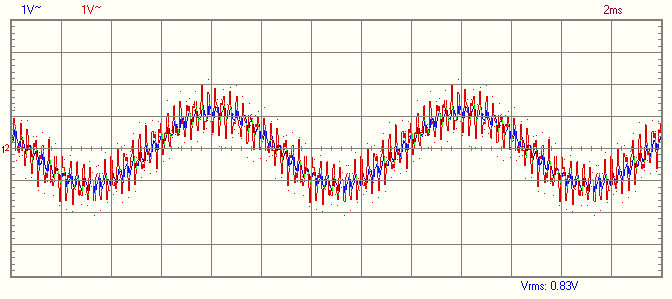
\includegraphics[width=.8\textwidth]{files/aufgabe8_teil2_tiefpass_oszi.png}
  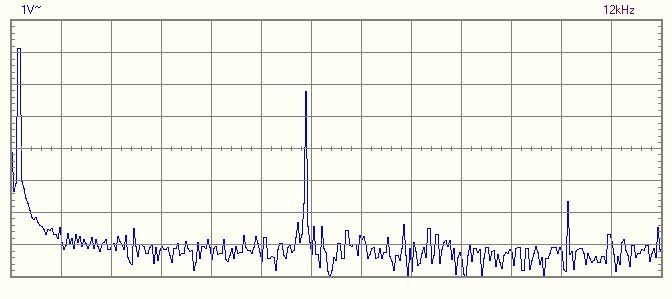
\includegraphics[width=.8\textwidth]{files/aufgabe8_teil2_tiefpass_spectrum.png}
  \caption{Ein- (rot) und Ausgangsspannung (blau) und Frequenzspektrum des überlagerten Signals mit Tiefpassfilter.}
  \label{fig:aufgabe8_teil2_tiefpass}
\end{figure}

Auch hier betrachten wir noch einmal die Dämpfung der einzelnen Signalanteile, zusammengefasst in \tabref{tab:dmpf_tiefpass}.

\begin{table}[H]
  \centering
  \caption{Dämpfung der einzelnen Signalanteile beim $RC$-Tiefpassfilter.}
  \vspace*{1em}
  \label{tab:dmpf_tiefpass}
  \begin{tabular}{c|c|c|c}
    Signalanteil & Ungefilterte Amp. [dBV] & Gefilterte Amp. [dBV] & Dämpfung\\\hline
    100 Hz & $-3.06 \pm 0.02$ & $-2.75 \pm 0.02$ & $1.113 \pm 0.011$\\
    4 kHz & $-8.06 \pm 0.02$ & $-15.88 \pm 0.02$ & $0.5076 \pm 0.0015$\\
    8 kHz & $-22.13 \pm 0.02$ & $-51.19 \pm 0.02$ & $0.4323 \pm 0.0005$
  \end{tabular}
\end{table}

%4kHz ValErr(-8.06, 0.02) ValErr(-15.88, 0.02) ValErr(0.5075566750629723, 0.001412385144501711)
%8kHz ValErr(-22.13, 0.02) ValErr(-51.19, 0.02) ValErr(0.4323109982418441, 0.0004256480161859309)
%100Hz ValErr(-3.06, 0.02) ValErr(-2.75, 0.02) ValErr(1.1127272727272728, 0.01088035483979233)

\newpage
\subsubsection*{$LC$-Tiefpassfilter}

\small{\textrightarrow\textit{Wir verwenden hier nun einen $47\si{\nano\farad}$ Kondensator.}}
\normalsize

Möchten wir das $8\si{\kilo\hertz}$-Signal weitestgehend unabhängig vom $4\si{\kilo\hertz}$-Signal dämpfen, benötigen wir einen Filter mit einem stärkeren Dämpfungsverlauf. Tauschen wir den Widerstand durch eine Spule aus, so erhalten wir einen $LC$-Tiefpassfilter, mit welchem genau dies erreicht werden kann. Dies spiegelt sich auch sehr deutlich im Spektrum (vgl. \abbref{fig:aufgabe8_teil2_lc_tiefpass}) wider. Der $8\si{\kilo\hertz}$-Anteil verschwindet nun quasi komplett im Untergrund, während das $4\si{\kilo\hertz}$ sehr deutlich hervorsticht. Es zeigt sich nun sogar eine Resonanzüberhöhung. Der $100\si{\hertz}$-Signalanteil ist jedoch weiterhin präsent, wie es auch bei einem Tiefpassfilter zu erwarten ist. Die Beobachtungen im Spektrum spiegeln sich auch, wie zuvor, sehr gut in der Signalformung des Ausgangssignals wider.

\begin{figure}[H]
  \centering
  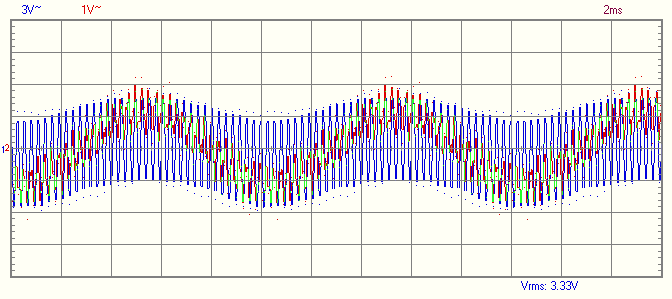
\includegraphics[width=.8\textwidth]{files/aufgabe8_teil2_lc_tiefpass_oszi.png}
  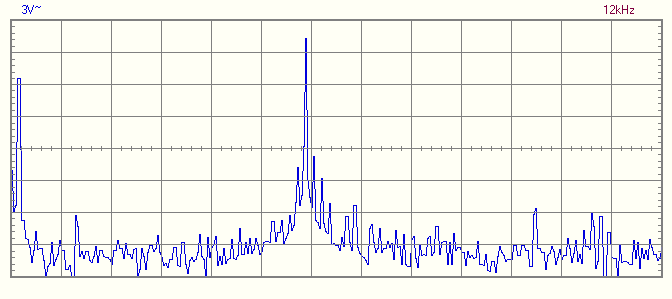
\includegraphics[width=.8\textwidth]{files/aufgabe8_teil2_lc_tiefpass_spectrum.png}
  \caption{Ein- (rot) und Ausgangsspannung (blau) und Frequenzspektrum des überlagerten Signals mit $LC$-Tiefpassfilter.}
  \label{fig:aufgabe8_teil2_lc_tiefpass}
\end{figure}

Bisher haben wir beobachtet, dass wir es mit den verwendeten Filterschaltungen nicht schaffen, das  $4\si{\kilo\hertz}$-Signal zu isolieren und nur die Signalanteile darum zu dämpfen. Bei der Verwendung eines Hoch- bzw. Tiefpassfilters ist dies auch klar, da diese ab ihrer Grenzfrequenz greifen und sich dann auf alle niedrigeren bzw. höheren Frequenzen auswirken. Um nur den Bereich um den $4\si{\kilo\hertz}$-Bereich durchzulassen, benötigen wir also einen Bandpassfilter, welchen wir uns in den folgenden Teilen anschauen.

\newpage
\subsubsection*{Bandpassfilter}

Zum Test des Bandpassfilters haben wir gleich mehrere Konfigurationen der RLC-Schaltung untersucht. Hierbei haben wir das Ausgangssignal je einmal an allen Bauteilen abgenommen und dies jeweils mit einem verbauten $1\si{\kilo\ohm}$- und einem $47\si{\ohm}$-Widerstand. Hieraus nehmen wir sechs verschiedene Resultate, also zwölf Plots mit. Um die Auswertung dieser abzukürzen, möchten wir uns hier auf das (subjektiv) beste Resultate beschränken.

\abbref{fig:aufgabe8_teil3_clR_47ohm_bandpass} zeigt das Signal bei Filterung durch einen RLC-Bandpassfilter mit $47\si{\ohm}$-Widerstand und Abnahme der Ausgangsspannung an selbigem. Wir können im Spektrum beobachten, dass der $8\si{\kilo\hertz}$-Signalanteil quasi komplett im Untergrund verschwindet. Auch der $100\si{\hertz}$-Anteil sticht nur noch leicht aus dem Untergrund hervor. Mittig ist nun, wie gewollt isoliert, der $4\si{\kilo\hertz}$-Anteil deutlich sichtbar. Auch die Signalform des Ausgangssignals zeigt, dass es sich quasi nur noch um eine einfache Sinusform ohne starke Überlagerungen handelt.


\begin{figure}[H]
  \centering
  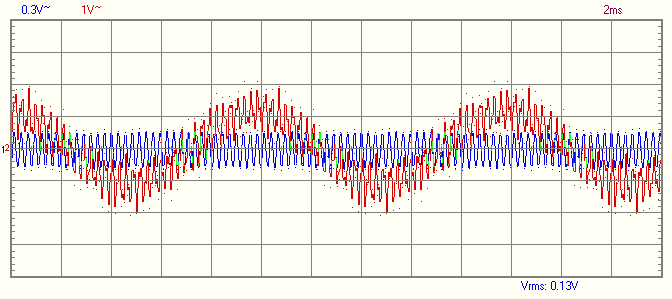
\includegraphics[width=.8\textwidth]{files/aufgabe8_teil3_clR_47ohm_bandpass_oszi.png}
  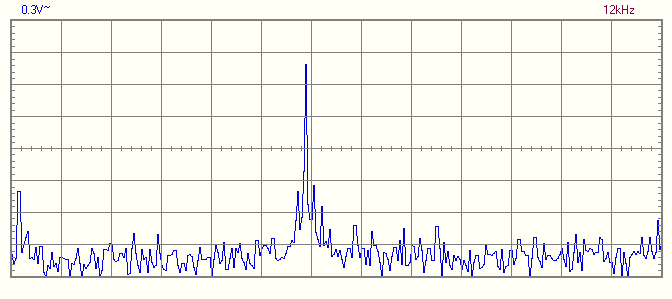
\includegraphics[width=.8\textwidth]{files/aufgabe8_teil3_clR_47ohm_bandpass_spectrum.png}
  \caption{Ein- (rot) und Ausgangsspannung (blau) und Frequenzspektrum des überlagerten Signals mit $RLC$-Bandpassfilter mit $47\si{\kilo\ohm}$ Widerstand, bei Spannungsabnahme über den Widerstand.}
  \label{fig:aufgabe8_teil3_clR_47ohm_bandpass}
\end{figure}
\newpage\noindent
Die Amplitude des $4\si{\kilo\hertz}$-Signalanteils liegt in dieser Konfiguration bei einem Wert von $-18.50 \pm 0.02 \mathrm{dBV}$. Dies entspricht im Vergleich zum ungefilterten Signal einer Dämpfung von
\begin{align}
  \frac{-8.06\mathrm{dBV}}{-18.50\mathrm{dBV}} = 0.4357 \pm 0.0012.
\end{align}

Im Vergleich dazu wird die Amplitude des $100\si{\hertz}$-Signals in dieser Filterschaltung auf $-57.56 \pm 0.02 \mathrm{dBV}$ gedämpft, was einer Dämpfung um
\begin{align}
  \frac{-3.06\mathrm{dBV}}{-57.56\mathrm{dBV}} = 0.0532 \pm 0.0004,
\end{align}
entspricht. Also einer deutlich stärkeren, als für das $4\si{\kilo\hertz}$-Signal.